\section{Multifrequency Multistage Radiolocation System}
\label{sec:mfms}
    This section explains \gls{mfms} in greater detail.
    Akin to other \gls{firl}s, \gls{mfms} consists of two main phases.
    During the offline phase, \gls{rss} information from anchor nodes is collected at many locations in the environment and used to approximate the radio wave propagation function.
    The online phase, on the other hand, makes use of the approximated propagation function obtained in the former phase.
    %  is used for localization purposes with new observations obtained at arbitrary locations.
    However, one major difference between \gls{mfms} and conventional \gls{firl} approaches is that \gls{mfms} employs three types of radio setups in three different stages to infer the location of the agent.

    The first stage of \gls{mfms}, localizes the agent with a grid-level accuracy based on \gls{lora} measurements, while the second stage employs WiFi and Bluetooth measurements separately to localize the agent within the grid attained in the former stage.
    The location estimates based on WiFi and Bluetooth measurements are fused into one final estimate.

    \begin{figure}[thpb]
        \centering
        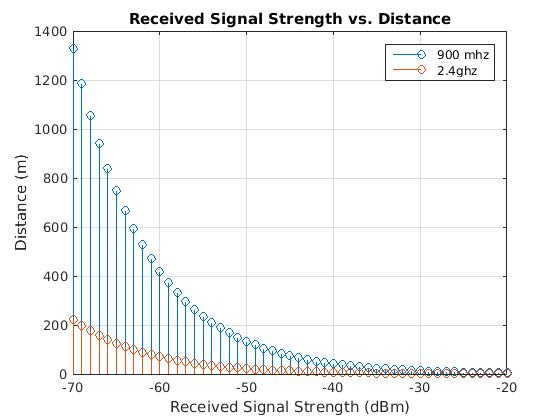
\includegraphics[width=\linewidth]{figures/rss-vs-distance.jpg}
        \caption{\label{fig:log-distance}\gls{rss} readings of two radio modules with same antenna characteristics are shown above. As the carrier frequency ($f_c = \frac{c}{\lambda}$) increases, the path loss shows the same trend. Thus, 900 MHz radios introduce a significantly bigger area of coverage comparing 2.4 GHz radios.}
    \end{figure}

    The main motivation behind employing multisource information is to exploit the diversity of the propagation characteristics of the different frequencies.
    As can be seen in the \Cref{eq:log-distance} and \Cref{fig:log-distance}, the received power and separation distance shows a log-linear relationship.
    %  demonstrates the log-distance relationship between received power and the separation between two antennas in two different frequencies in \gls{uhf} radio band.
    This figure implies two fundamental problems in radiolocation systems:
    The first problem is that as the carrier frequency increases path loss increases significantly, which limits the radio covarage and localization ability of the system in large environments.
    On the other hand, as the carrier frequency increases, the separation between two antennas, i.e.\ the anchor node and the target to be localized, can be identified with finer spatial resolution.
    Therefore, the trade-off between radio coverage and spatial localization resolution can be resolved by employing different frequencies in indoor localization systems by fusing the information acquired from the anchor nodes using different carrier frequencies.
    Thus, \gls{mfms} employs a \gls{lora} (900 MHz), a WiFi \gls{ap} and a Bluetooth (2.4 GHz) beacon in each anchor node.
    \Cref{tab:specs} tabulates the specifications of the radios consisting in each anchor node, while \Cref{fig:module} demonstrates the details of the anchor nodes.
    In other words, wider spatial coverage is achieved by using \gls{lora} modules working at 900 MHz while finer spatial resolution provided by WiFi and Bluetooth both working at 2.4 GHz frequency.

    \begin{table}
    \begin{center}
    \caption{\label{tab:specs}The specifications of radios used in anchor nodes}
      \begin{tabular}{@{}lccc@{}}\toprule[1.5pt]
        Property                        &WiFi           &Bluetooth      &\gls{lora}\\ \midrule[1.5pt]
        Frequency [MHz]:                &2400           &2400           &900 \\ \midrule
        Communication Bandwidth:        &1-11 Mbps      &Upto 4 Mbps    &10 Kbps \\ \midrule
        Transmission Power $P_t$ [dBm]: &17             &10             &24 \\ \midrule
        Reciever Sensivity [dBm]:       &?              &-98            &-101 \\ \midrule
        Communication Range [m]:        &$<$20          &$~$10            &$>$100  \\\bottomrule[1.5pt]
      \end{tabular}
    \end{center}
    \end{table}

    \begin{figure}[thpb]
       \centering
       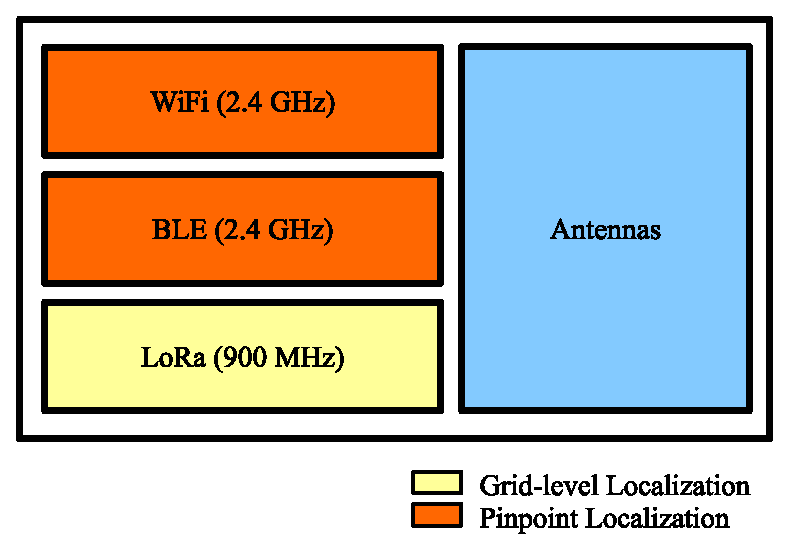
\includegraphics[width=0.8\linewidth, scale=0.6]{figures/mfms_module.eps}
       \caption{\label{fig:module}\gls{mfms} Anchor Nodes}
    \end{figure}

    \subsection{Stage 1:Spatially-coherent Path Loss Exponent Estimation}
    This section covers the details of the joint path loss exponent estimation which forms the first stage of \gls{mfms}.
    \gls{mfms} approaches the \gls{firl} problem in the scope of curve fitting.
    However, unlike many proposed approaches mentioned earlier, \gls{mfms} does not solely rely on the collected data to fit a function which best explains the training data given the location labels.
    Moreover, \gls{mfms} does not consider the path loss exponent as a variable describing the whole localization environment.
    Instead, we approach the problem by estimating a path loss exponent for different regions in the environment.
    %  differing in value depending on the regions at which the agent resides.
    In other words, the path loss exponent for \gls{mfms} is a function of the region at which the agent might reside.
    Therefore, the proposed system is able to tackle multi-modal propagation caused by non-uniform distribution of obstructions in the environment.

    \begin{figure}[thpb]
       \centering
       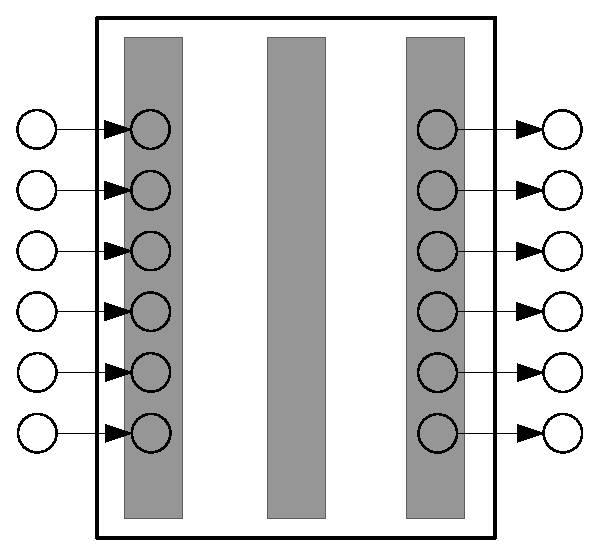
\includegraphics[width=\linewidth]{figures/softmax.eps}
       \caption{\label{fig:softmax}The softmax classifier assigns weights for each anchor node based on the evidence representing the probability of residing in a grid cell $g$.}
    \end{figure}

    Let $\Omega=\{g_\theta | \theta=1\ldots n_{grid}\}$ be the localization environment which is divided into $n_{grid}$ number of grid cells $g$.
    Spatially-coherent path loss exponent $n^{*,i}_g$, which is the path loss exponent of anchor node $i$ in grid cell $g$, can be formulated in least square sense by using the \gls{ldpl} model.
    \begin{equation}
       n^{*,i}_g = \argmin_n{\sum_{j_g} \left(d^i_{j_g} - f_d(m^i_{j_g},n)\right)^2}
    \end{equation}
    where $d^i_{j_g}$ and $m^i_{j_g}$ denote the radial distance between anchor node $i$ and the measurement location with in grid cell $g$, and the measurements acquired in grid cell $g$, while $f_d(\cdot)$ denotes the \gls{ldpl} model.
    This estimation is conducted once during the offline phase from the collected fingerprints; while, during the online phase, the estimated spatially-coherent path loss exponents are chosen from $\bm{n}^{*,i} =\{n^{*,i}_g | g=1\ldots n_{grid}\}$ according to the belief of the agent resides in the grid cell $g$.
    During the online phase, the selection of \gls{mfms} first localizes the agent's vicinity with a grid-level accuracy by employing a softmax classifier which is depicted in \Cref{fig:softmax}.
    The classifier assigns a probability of the agent might reside to each grid cell given the acquired \gls{lora} measurements.
    The reason \gls{mfms} solely employs \gls{lora} measurements in grid-level localization is that due to the higher probability of observing multiple \gls{lora} modules in arbitrary positions in the environment, thanks to the smallar path loss they introduce.
    During online phase, the estimated spatially-coherent path loss exponent, a set of physical parameter defining the radio wave propagation, is incorporated into the location estimation process in Stage-II\@.

    % Because the spatially-coherent path loss exponent is a function of the grid cells, grid-level localization should be accomplished during online phase so that the proper spatially-coherent path loss exponent can be chosen.
    % The weights of each grid is learned with a softmax classifier, which is depicted in \Cref{fig:softmax}.


    \subsection{Stage 2:Pinpoint Localization}
    This section gives details of the second stage of the \gls{mfms} which is the pinpoint localization.
    After obtaining the spatially-coherent path loss exponent corresponding to a grid cell, the agent is localized within the grid cell with finer spatial-resolution.
    This pinpoint localization process relies on the approximation joint propagation function of all the anchor nodes.
    Instead of independently modeling each anchor node, \gls{mfms} models all the propagation of functions jointly.

    During the offline phase, the joint propagation function $\hat{g}_d(\cdot)$ is approximated with the collected fingerprints.
    The approximated joint propagation function is formulated as below.
    % , which $\mathbb{Z}^{n_{node}\times n_m} \mapsto \mathbb{R}^2$:
    % Similar to \gls{ldpl}, our radio wave function approximation is given below:
    \begin{equation}
        \label{eq:propfunct}
        \hat{g}_d(\bm{m}^{k-n_{m}:k}_j, \bm{n}^*_g)= \bm{\hat{x}}
    %   n(k,t)^* = \argmin_n \bm{e}^i  = \argmin_n \{d^i_j - \hat{f}^i_d(m_i, n, t)\}
    \end{equation}
    where $\bm{m}^{k-n_{m}:k}_j \in \mathbb{R}^{n_{node} \times n_m}$, $\bm{n}^*_g \in \mathbb{R}^n_{node}$, and $\bm{\hat{x}}$ are the measurement vector acquired from all anchor nodes between time steps $k-n_m$ and $k$, the estimated path loss exponent vector of each anchor node for grid cell $g$ and the estimated absolute position of the agent, respectively.
    As can be seen in \Cref{eq:propfunct}, the joint propagation function incorporates the measurements with the spatially-coherent path loss exponent vector so that the physical characteristics of the radio waves, represented with the path loss vector, are enforced into the model as a parameter.

    \begin{figure}[thpb]
       \centering
       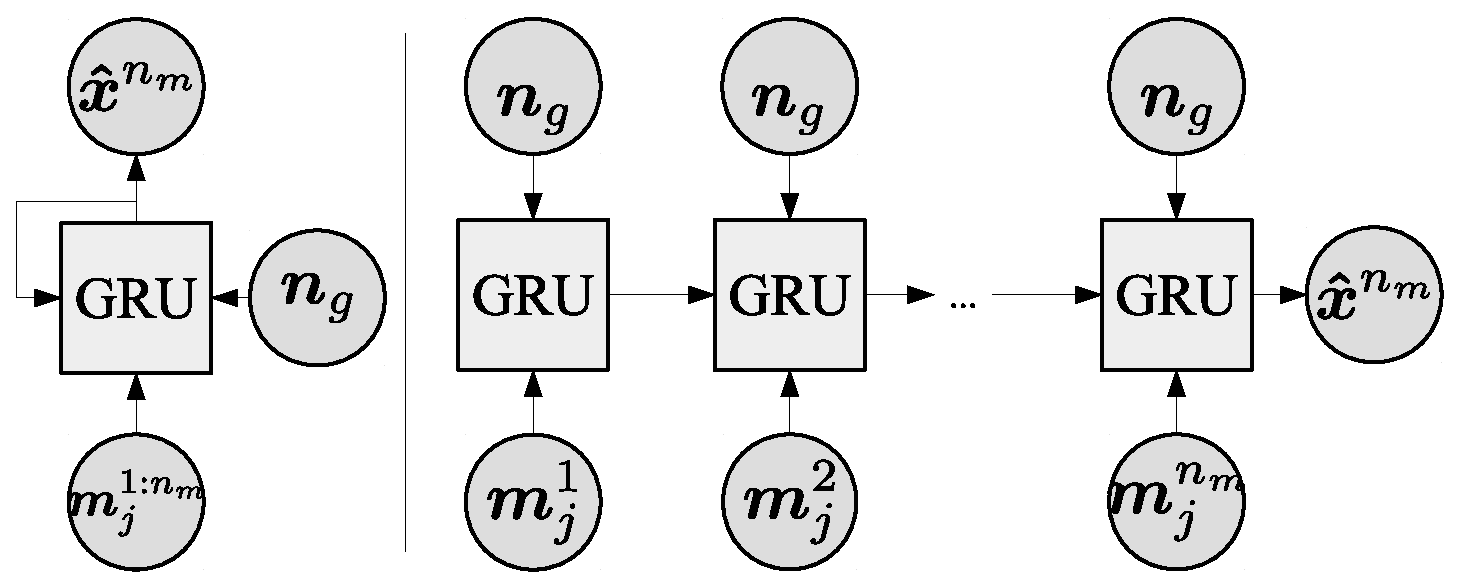
\includegraphics[width=0.9\linewidth]{figures/gru.eps}
       \caption{\label{fig:gru}Left: Folded \gls{gru}. Right: Unfolded \gls{gru}.}
    \end{figure}

    The propagation function of WiFi $\hat{g}^w_d(\cdot)$ and Bluetooth $\hat{g}^b_d(\cdot)$ anchors are approximated with two independent recurrent neural networks, consisting of three layers of \gls{gru}~\cite{cho2014learning}.
    Unlike conventional \gls{nn} architectures, the recurrent neural networks are able to exploit information in form of sequences, i.e.\ the result of previous input affects the latter input.
    This ability is enables \gls{mfms} to exploit the temporal coherence of the radio waves and the physical limitations of the agents motion model.
    In other words, the estimation during the time step $k$ should consider the estimation result of time step $k-1$.
    \Cref{fig:gru} depicts a layer of \gls{gru} model in folded and unfolded representation.
    As can be seen in the figure, the \gls{gru} model recursively incorporates the each temporal slice of the input.

    These functions are attained with a \gls{sgd} based back-propagation algorithm.
    During the online phase of the \gls{mfms}, the approximated joint propagation functions are employed to estimate the location of the agent.
    Specifically, the pinpointing algorithm incorporates the spatially-coherent path loss exponent along with the weighted measurements to estimate $\bm{\hat{x}}^w$ and $\bm{\hat{x}}^b$, estimated positions by using WiFi measurements and Bluetooth measurements, respectively.

    % The locatization environment is divided into $n_{grid}$ number of grids in order to obtain


    \subsection{Stage 3:Information Fusion}
    This section of the paper further explains the Stage-III of the \gls{mfms}.
    The Stage-III is essentially an information fusion layer of the model where location estimates of WiFi and Bluetooth measurements are fused into one final entity.
    The incorporation of two estimates are achieved in the framework of a \gls{nn} consisting of 3 layers.
    The network is in a gradually narrowing structure such that the first, second and last layer contain 8, 4, 2 neurons, respectively.
    \Cref{fig:fusion} demonstrates the Phase-III\@.

    \begin{figure}[thpb]
       \centering
       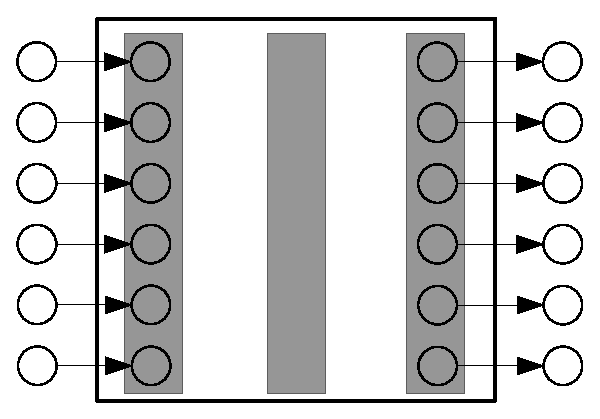
\includegraphics[width=0.95\linewidth]{figures/fusion.eps}
       \caption{\label{fig:fusion}Two location estimates of WiFi and Bluetooth approximations are fused with a 3 layered-\gls{nn}.}
    \end{figure}
